% !Mode:: "TeX:UTF-8"
%%%%%%%%%%%%%%%%%%%%%%%%%%%%%%%%%%%%%%%%%%%%%%%%%%%%%%%%%%%%%%%%%%%%%%%%%%%%%%%%
%          ,
%      /\^/`\
%     | \/   |                CONGRATULATIONS!
%     | |    |             SPRING IS IN THE AIR!
%     \ \    /                                                _ _
%      '\\//'                                               _{ ' }_
%        ||                     hithesis v3                { `.!.` }
%        ||                                                ',_/Y\_,'
%        ||  ,                   dustincys                   {_,_}
%    |\  ||  |\          Email: yanshuoc@gmail.com             |
%    | | ||  | |            https://yanshuo.site             (\|  /)
%    | | || / /                                               \| //
%    \ \||/ /       https://github.com/dustincys/hithesis      |//
%      `\\//`   \\   \./    \\ /     //    \\./   \\   //   \\ |/ /
%     ^^^^^^^^^^^^^^^^^^^^^^^^^^^^^^^^^^^^^^^^^^^^^^^^^^^^^^^^^^^^^^
%%%%%%%%%%%%%%%%%%%%%%%%%%%%%%%%%%%%%%%%%%%%%%%%%%%%%%%%%%%%%%%%%%%%%%%%%%%%%%%%
\documentclass[fontset=fandol,toc=true,type=master,stage=opening,campus=shenzhen]{hithesisart}
% 此处选项中不要有空格
%%%%%%%%%%%%%%%%%%%%%%%%%%%%%%%%%%%%%%%%%%%%%%%%%%%%%%%%%%%%%%%%%%%%%%%%%%%%%%%%
% 必填选项
% type=doctor|master|bachelor
% stage=opening|midterm
%%%%%%%%%%%%%%%%%%%%%%%%%%%%%%%%%%%%%%%%%%%%%%%%%%%%%%%%%%%%%%%%%%%%%%%%%%%%%%%%
% 选填选项(选填选项的缺省值已经尽可能满足了大多数需求,除非明确知道自己有什么
% 需求)
% campus=shenzhen|weihai|harbin
%   含义:校区选项,默认harbin
% fontset=windows|mac|ubuntu|fandol
%   含义:前三个对应各自系统,fandol是开源字体。
% toc=true|false
%   含义:是否显示目录,默认true
% newtxmath=true|false
%    含义:是否使用 times 风格数学字体,默认true
% print=true|false
%   含义:是否在封面后增加一个空白页用于打印,默认false
%%%%%%%%%%%%%%%%%%%%%%%%%%%%%%%%%%%%%%%%%%%%%%%%%%%%%%%%%%%%%%%%%%%%%%%%%%%%%%%%
\usepackage{bm}

\graphicspath{{figures/}}


\begin{document}

% !Mode:: "TeX:UTF-8"

\hitsetup{
  %******************************
  % 注意:
  %   1. 配置里面不要出现空行
  %   2. 不需要的配置信息可以删除
  %******************************
  ctitlecover={基于视觉惯性的全驱动旋翼无人机状态估计与导航研究},%放在封面中使用,自由断行
  % ctitleone={局部多孔质气体静压},
  % ctitletwo={轴承关键技术的研究},
  caffil={机电工程与自动化学院},
  csubject={控制科学与工程},
  cauthor={刘培焱},
  cstudentid={22S053073},
  cclassid={},
  csupervisor={陈浩耀教授},
  % 日期自动使用当前时间,若需指定按如下方式修改:
  %cdate={盘古开天地}
  % cenrolldate={公元2020年}
}

\makecover

% 深圳博士开题报告 -----------------------------------------------

% !Mode:: "TeX:UTF-8"
%%%%%%%%%%%%%%%%%%%%%%%%%%%%%%%%%%%%%%%%%%%%%%%%%%%%%%%%%%%%%%%%%%%%%%%%%%%%%%% 
%                          _
%  _____ ____ _ _ __  _ __| |___ ___
% / -_) \ / _` | '  \| '_ \ / -_|_-<
% \___/_\_\__,_|_|_|_| .__/_\___/__/
%                    |_|
%  _              _         _   _
% | |__ _  _   __| |_  _ __| |_(_)_ _  __ _  _ ___
% | '_ \ || | / _` | || (_-<  _| | ' \/ _| || (_-<
% |_.__/\_, | \__,_|\_,_/__/\__|_|_||_\__|\_, /__/
%       |__/                              |__/
%%%%%%%%%%%%%%%%%%%%%%%%%%%%%%%%%%%%%%%%%%%%%%%%%%%%%%%%%%%%%%%%%%%%%%%%%%%%%%%
\section{课题来源及研究的目的和意义}
\subsection{研究背景}
进入21世纪以来,多旋翼无人机领域取得了很大的发展。
为突破现在市场上主流的欠驱动无人机所存在的瓶颈,近年来人们又研制出了不少种的全驱动多旋翼无人机系统,
这种无人机可以跟踪6自由度轨迹,有效增强了多旋翼无人机的机动性能,拓宽了其应用场景。

作为一个高自由度且敏捷的系统,无人机的稳定自主飞行依赖鲁棒且高精度的导航系统来对自身和外界的状态进行有效估计。
同时定位与建图(Simultaneous Localization and Mapping, SLAM)技术\cite{liu2016asurvey}被广泛应用于移动机器人的实时定位导航中,
使得机器人在复杂的无GPS环境中也能获得准确的状态估计和环境感知。
其中,基于视觉或视觉惯性融合的SLAM导航技术(VSLAM或VISLAM)以其相对较低的成本、轻量级的硬件需求和较高的精度和鲁棒性成为适用于无人机的选择。

\subsection{研究的目的及意义}
% 视觉-惯性导航
移动机器人导航一直以来被广泛研究。
目前常用的导航方式是基于全球导航卫星系统(Global Navigation Satellite System, GNSS)的,
但是这种方法并不适用与室内、隧道等卫星信号质量差的环境。
SLAM技术则很好地弥补了基于GNSS的导航系统的局限性,
其具体是指搭载特定传感器的主体,在没有环境先验信息的情况下,于运动过程中建立环境的模型,同时估计自己的运动\cite{davison2007monoslam}。
可见传感器的选择是研究和实现SLAM技术的重点。

\begin{figure}[!ht]
    \setlength{\subfigcapskip}{-1bp}
    \centering
    \begin{minipage}{\textwidth}

    \centering
    \subfigure{\label{subfig:rgbd_camera}}\addtocounter{subfigure}{-2}
    \subfigure{\subfigure[深度相机]{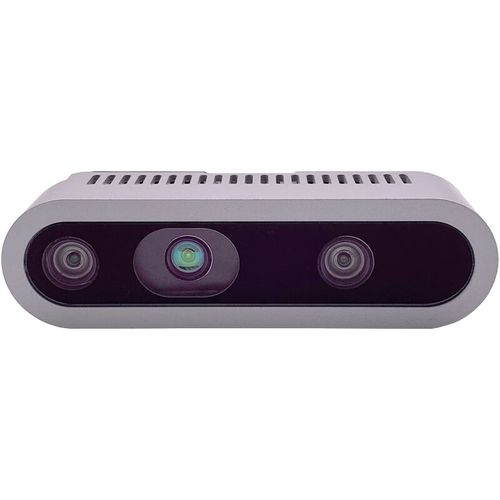
\includegraphics[width=0.32\textwidth, height=0.32\textwidth]{visual_sensor.jpeg}}}
    \subfigure{\label{subfig:imu}}\addtocounter{subfigure}{-2}
    \subfigure{\subfigure[IMU]{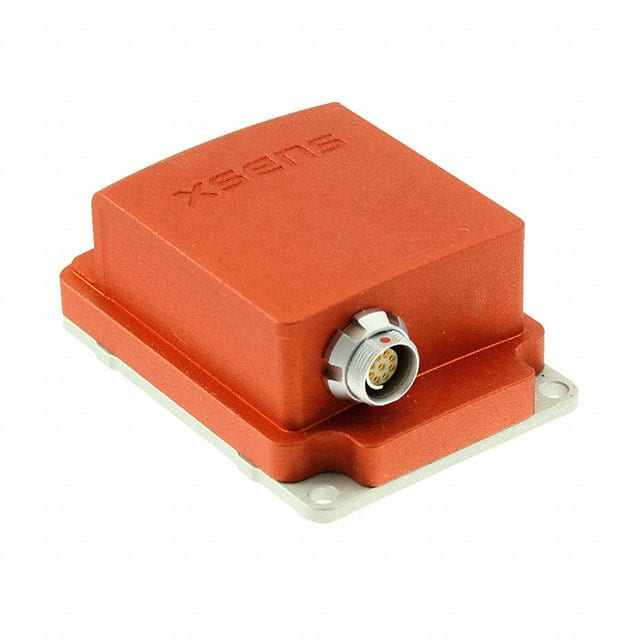
\includegraphics[width=0.32\textwidth, height=0.32\textwidth]{inertial_sensor.jpeg}}}
    \subfigure{\label{subfig:lidar}}\addtocounter{subfigure}{-2}
    \subfigure{\subfigure[激光雷达]{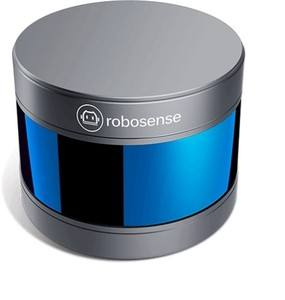
\includegraphics[width=0.32\textwidth, height=0.32\textwidth]{lidar.jpeg}}}

    \end{minipage}
    \caption{SLAM技术常用的传感器}
    \label{fig:common_sensors_for_slam}
\end{figure}

如图\ref{fig:common_sensors_for_slam}所示目前SLAM系统中常用的传感器有相机(视觉传感器)、惯性测量单元(Inertial Measurement Unit, IMU)和激光雷达等。
基于IMU的惯性导航是一项很经典的技术,并且已经发展得相当成熟,利用IMU提供的高频6DoF运动信息可以非常精确地估计姿态,
但是受IMU中陀螺仪和加速度计的零漂和噪声的影响,在积分求解位置的时候不可避免地会产生误差累积和漂移(drift),
因此,IMU一般不会单独用作SLAM的传感器。
基于激光雷达的SLAM导航技术也已经发展地比较成熟,但是激光雷达的体积和重量较大,而且成本较为高昂。
相对而言视觉传感器体积小、重量轻、成本低,并且能提供更为丰富的环境信息,这些特性使得视觉SLAM技术一直以来是学术界研究的热点。
然而视觉传感器同时也存在难以恢复尺度信息(主要针对于单目视觉)、低频、对光照敏感等问题。
实际上,在较为复杂的场景下仅靠单一的传感器是难以实现理想的导航定位效果的,
在这样的背景下,融合IMU和视觉信息的视觉-惯性导航系统(Visual-Inertial Navigation Systems, VINS)成为一个重要的研究课题。
VINS保留了纯视觉SLAM的小体量和低成本,并且结合了IMU和相机二者的优点,变得更加鲁棒和精确,在敏捷且追求轻量化的无人机系统上具有很高的研究价值和广阔的应用前景。

% 全驱动无人机
多旋翼无人机的驱动力包括3维的推力$\bm{f} \in \mathbb{R}^3$和3维的力矩$\bm{\tau} \in \mathbb{R}^3$,
可将二者合并为一个6维向量$\bm{w} = \left[\bm{f}^\top \quad \bm{\tau}^\top\right]^\top \in \mathbb{R}^6$称为力螺旋(wrench)。
产生驱动力的执行器指令组成控制输入$\bm{u} \in \mathbb{R}^{n_{\bm{u}}}$。
由给定力螺旋$\bm{w_\text{act}}$求解对应控制输入$\bm{u}$的过程称为控制分配(control allocation),
如图\ref{fig:uav_classification}所示,我们按照执行器雅可比(Jacobian)$\frac{\partial \bm{w_\text{act}}}{\partial \bm{u}} \in \mathbb{R}^{6 \times n_{\bm{u}}}$的秩可将无人机分为欠驱动系统和全驱动系统\cite{bodie2022omnidirectional}。
目前常用的平行轴四旋翼、六旋翼等传统无人机属于欠驱动系统,它们的控制分配雅可比的秩为4,意味着它们只有4个控制自由度,
导致其机动性受限,且抗干扰能力弱。
为解决这些问题,充分发挥多旋翼飞行器的潜力,近年来发展出了多种全驱动无人机。
这些工作通过改变旋翼几何构型、增加旋翼倾转自由度等方式让旋翼能提供相对机身任意方向的推力和转矩,使得$\text{rank}(\frac{\partial \bm{w}_\text{act}}{\partial \bm{u}}) = 6$。
全驱动无人机能够独立地进行位置和姿态控制,具有任意姿态悬停、跟踪6自由度全状态轨迹的能力,故又称为全向飞行器(omnidirectional aerial vehicle)。
进行这种受控的、自由的刚体运动是传统欠驱动多旋翼飞行器所无法做到的,这也赋予了全驱动无人机在空中作业、避障等方面很大的优势和潜力。

\begin{figure}[htbp]
    \centering
    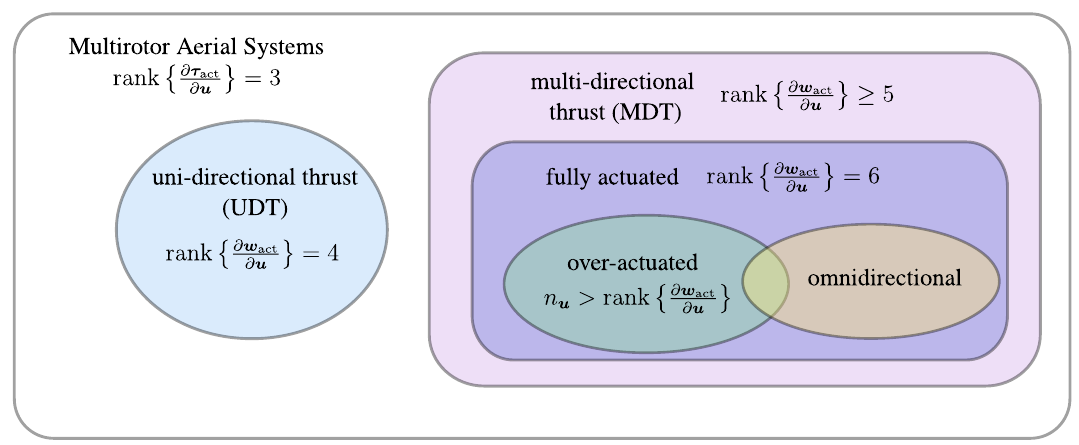
\includegraphics[width = \textwidth]{figures/uav_classification.png}
    \caption{无人机系统的分类\cite{bodie2022omnidirectional}}
    \label{fig:uav_classification}
\end{figure}

% 无人机外力估计
作用在无人机上的外力(external wrench)可以等效分解为作用在无人机质心上的合外力(external force)和外力矩(external torque),
合外力对无人机的平移动力学产生扰动,外力矩则对无人机的旋转动力学产生扰动,
这些扰动的来源可能有风扰、接触、机上载荷(如机械臂)以及空气动力学效应(如狭小空间中的乱流)等,
可能会严重影响无人机的正常作业。
为了补偿这些扰动,无人机的控制模块和规划模块需要精确地知晓合外力和外力矩的大小和方向\cite{ding2021vid},
对于具有独立控制6自由度力和力矩能力的全驱动无人机而言,其具有比传统欠驱动无人机更优秀的扰动补偿能力。
因此,有必要为全驱动无人机设计一个显示考虑外力的状态估计器。

本课题的目标是设计一个基于视觉惯性融合的SLAM导航系统,
期望此系统能够:

(1) 精确且高效地估计自身运动。

(2)能结合无人机的动力学模型精确且高效地估计外部作用力。
 
(3)适用于全驱动无人机,并能结合建图与规划模块实现自主导航。

% \begin{enumerate}
%     \item 精确且高效地估计自身运动;
%     \item 能结合无人机的动力学模型精确且高效地估计外部作用力;
%     \item 适用于全驱动无人机,并能结合建图与规划模块实现自主导航。
% \end{enumerate}

\section{国内外研究现状及分析}

\subsection{国内外研究现状}
\subsubsection{视觉SLAM及视觉惯性SLAM导航研究现状}\label{subsubsec:status_of_vslam_and_vislam}

\begin{figure}[htbp]
    \centering
    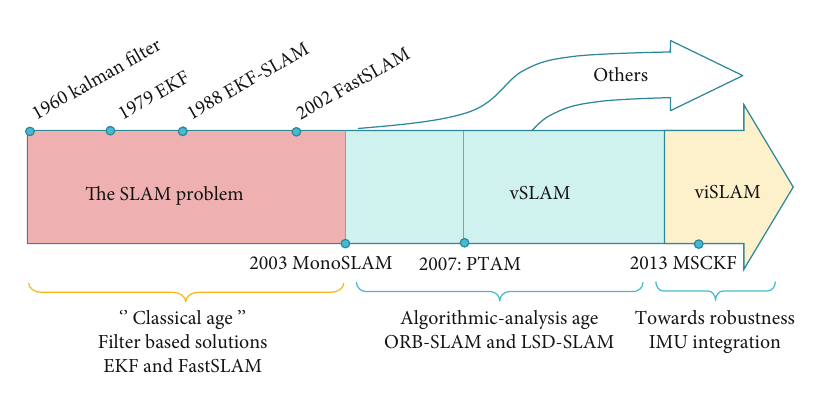
\includegraphics[width = \textwidth]{figures/vslam_history.png}
    \caption{视觉SLAM和视觉惯性SLAM发展的3个阶段\cite{servieres2021visual}}
    \label{fig:vslam_history}
\end{figure}

VSLAM和VISLAM到当下已经取得了长足的发展,
如图\ref{fig:vslam_history}所示,整个发展历史大致可分为3个阶段\cite{servieres2021visual}:
第一阶段被称为“古典时期(the classical age)”,
这一时期的SLAM研究者们主要专注于解决SLAM问题。
一些相关的数学公式被提出,SLAM首次得到了高效地应用。
在第二阶段(图\ref{fig:vslam_history}中的Algorithmic-analysis age),SLAM研究的焦点转移到了基于视觉的方法(vision-based approaches),
此阶段也被称为SLAM研究的“黄金阶段”\cite{servieres2021visual}。
这期间研究者们提出了一些视觉SLAM方案,并且将GPU、RGB-D相机、双目相机(stereo camera)等新型硬件集成到了SLAM系统中。
视觉SLAM的一些重要性质(如收敛性和一致性)也得到了研究,
也是从这个时期开始视觉SLAM成为了SLAM方法发展的中心。
第三阶段视觉SLAM的研究主要致力于改善系统的鲁棒性(robustness),
目标在于提高视觉SLAM系统的可靠性以支持日益增长的实际应用需求(如无人机、虚拟现实等),
视觉惯性SLAM也是在这个时期被引入的。

时至今日,视觉SLAM和视觉惯性SLAM的研究取得了丰硕的成果,
已经有许多优秀的框架诞生:
视觉SLAM领域有LSD-SLAM\cite{engel2014lsd}、ORB-SLAM2\cite{mur2017orb}、DSO\cite{engel2017direct}等,
视觉惯性SLAM领域有VINS-Mono\cite{qin2018vins}、ORB-SLAM3\cite{campos2021orb}、DM-VIO\cite{von2022dm}等。
这些极大地推动了机器人导航定位技术的发展。

\subsubsection{无人机的外力估计研究现状}\label{subsubsec:external_wrench_estimation}
无人机的外力估计也是一个被研究多年的课题,并且当下已有多种多样的解决方案,
大致上可以分为确定性方法、概率性方法和基于滑窗(sliding window)优化的方法\cite{nisar2019vimo}。
特别是近年发展出的无人机动力学模型辅助的视觉惯性SLAM方法\cite{ding2021vid, nisar2019vimo},
该方法将外力也作为VIO系统的待估计变量,
根据动力学模型构造动力学残差项并将其添加进后端优化的代价函数中。
结果表明这种方法既可以紧耦合地精确估计外力、又可以提高原VIO部分的精度,
有待改进的一点是该方法只能估计三维合外力而不能估计外力矩,
然而外力矩的估计对于无人机(特别是全向无人机)来说也具有重要意义。
视觉、惯性和动力学模型三者紧耦合的运动和外力估计也是本课题将重点探索的方向。

\subsubsection{全驱动旋翼无人机研究现状}

\begin{figure}[!ht]
    \setlength{\subfigcapskip}{-1bp}
    \centering
    \begin{minipage}{\textwidth}

    \centering
    \subfigure{\label{subfig:fix_rotor}}\addtocounter{subfigure}{-2}
    \subfigure{\subfigure[固定旋翼型\cite{brescianini2016design}]{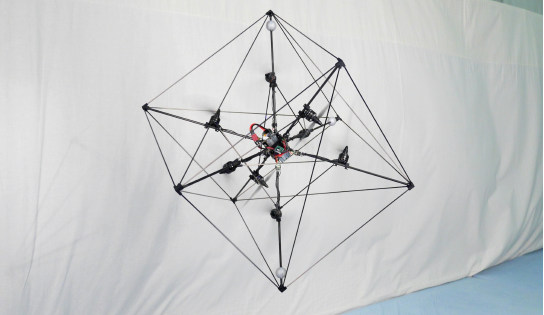
\includegraphics[width=0.45\textwidth]{octo_omav.png}}}
    \subfigure{\label{subfig:tilt_rotor}}\addtocounter{subfigure}{-2}
    \subfigure{\subfigure[倾转旋翼型\cite{kamel2018voliro}]{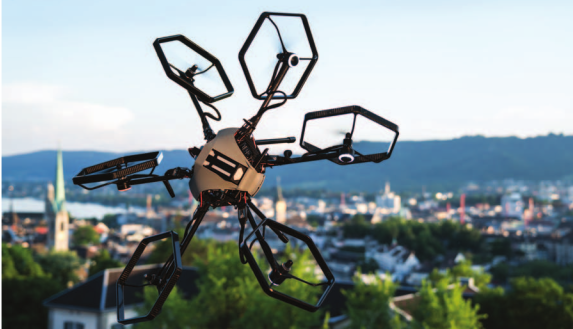
\includegraphics[width=0.45\textwidth]{voliro_2.png}}}

    \end{minipage}
    \caption{两种类型的全驱动旋翼无人机}
    \label{fig:two_types_of_fully_actuated_uav}
\end{figure}

实现多旋翼飞行器全驱动化的要点在于使驱动器同时且独立地产生相对机体任意方向推力和力矩,而要做到这一点需要改变旋翼的构型(configuration of rotors)。
全驱动多旋翼飞行器领域近年来正处于持续发展中,这些飞行器按照旋翼构型大致可分为两类:固定旋翼型(fixed-rotor)\cite{brescianini2016design, park2018odar,allenspach2020design}和倾转旋翼型(tiltrotor)\cite{ryll2014novel, kamel2018voliro}。
图\ref{fig:two_types_of_fully_actuated_uav}分别展示了两种构型中具有代表性的一项工作。

\subsection{国内外文献综述及简析}
\subsubsection{视觉SLAM及视觉惯性SLAM文献综述及简析}
卡尔曼滤波(Kalman Filter)\cite{kalman1960new}和扩展卡尔曼滤波(Extended Kalman Filter, EKF)\cite{maybeck1982stochastic}的提出开启了现代定位(localization)的研究历史。
SLAM问题在20世纪80年代成形,并且于1995年证明了收敛性\cite{durrant1988uncertain,leonard1991simultaneous,smith1986representation}。
在这段时间里,一些SLAM方法被提出,它们主要基于激光测距仪及从不同来源计算的里程计信息,并且基于EKF实现,
如Smith等人于1988年提出的EKF-SLAM\cite{cheeseman1987stochastic}。
Davison等人于2007年提出的MonoSLAM\cite{davison2007monoslam}是第一个只用单个低成本的视觉传感器的SLAM方法,
其仅用一个网络摄像头、一台通用电脑,并且不需要里程计的测量值,就实现了基于EKF的3维建图和定位。
至此基于视觉的SLAM研究进入了\ref{subsubsec:status_of_vslam_and_vislam}节中提到的“黄金阶段”。

本小节接下来分别对视觉SLAM和视觉惯性SLAM技术进行文献综述及简析。

(1)视觉SLAM

\begin{figure}[htbp]
    \centering
    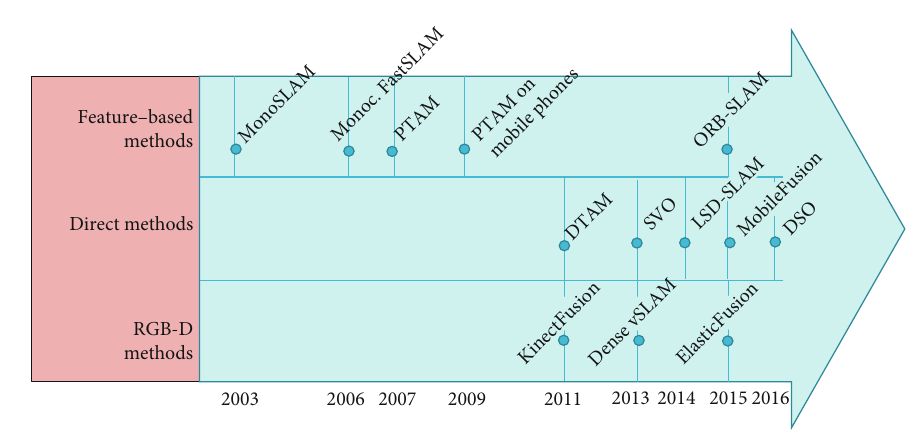
\includegraphics[width = \textwidth]{figures/vslam_classification.png}
    \caption{视觉SLAM方法分类\cite{servieres2021visual}}
    \label{fig:vslam_classification}
\end{figure}

如图所示,一般将视觉SLAM方法根据其输入数据的本质分为3类\cite{servieres2021visual}:
特征点法(feature-based methods)、直接法(direct methods)和RGB-D法(RGB-D methods)。

\begin{figure}[htbp]
    \centering
    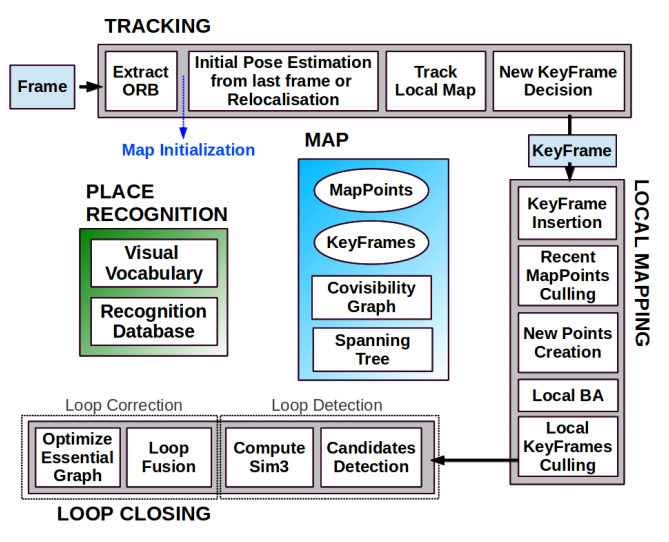
\includegraphics[width = 0.8\textwidth]{figures/orb_slam_system_overview.png}
    \caption{ORB-SLAM系统框架图\cite{mur2015orb}}
    \label{fig:orb_slam_system_overview}
\end{figure}

\textbf{特征点法}:
特征点法依赖于特征点的提取与匹配,它具有稳定,对光照和动态物体不敏感的优势。
目前常用的特征点方案有Harris\cite{si1988combined}、SURF\cite{bay2006surf}、SIFT\cite{lowe2004distinctive}、FAST\cite{rosten2006machine}和ORB\cite{rublee2011orb}等,
特征点方案的选择主要取决于对鲁棒性和计算效率的权衡。
前述的MonoSLAM\cite{davison2007monoslam}是一种基于EKF的特征点法视觉SLAM。
基于EKF的特征点法SLAM都会受到特征点数量平方级的复杂度的困扰。
2002年,Rao-Blackwellized粒子滤波器(particle filter)被应用于Montemerlo等人提出的FastSLAM\cite{montemerlo2002fastslam},
该方法有效降低了对数尺度的复杂性(the complexity of logarithmic scaling),并且被成功迁移到了单目视觉SLAM中\cite{eade2006scalable}。
然而,即使是FastSLAM方法的最小复杂度也严重限制了SLAM的应用,
尤其是需要提取大量特征点的视觉SLAM。
直到2007年,Klein等人提出了一种基于关键帧的(keyframe-based)解决方案PTAM\cite{klein2007parallel},
该方案基于FAST特征点,实现了任务并行化,更好地利用了全局优化技术,减小了跟踪漂移,
并且更重要的一点是实现了一种具有自由缩放性的特征存储方法。
现今几乎所有的视觉SLAM算法都是基于PTAM的概念。
Mur-Artal等人于2015年基于ORB特征点提出了成为现代主流视觉SLAM框架之一的ORB-SLAM\cite{mur2015orb}。
ORB-SLAM通过引入回环检测(loop detection)和重定位(relocalization),
实现了长时间尺度上的数据关联,减小了累积误差。
ORB-SLAM模块划分清晰,成为很多后续工作的基础,
其系统框架如图\ref{fig:orb_slam_system_overview}所示,
后续的ORB-SLAM2\cite{mur2017orb}和ORB-SLAM3\cite{campos2021orb}(属于视觉惯性SLAM)都是在其基础上的改进。
除了基于特征点,也有一些引入线特征的视觉SLAM方案,
如2017年Pumarola等人提出的PL-SLAM\cite{pumarola2017pl}、2018年He等人提出的PL-VIO\cite{he2018pl}(属于视觉惯性SLAM)和2020年Fu等人提出的PL-VINS\cite{fu2020pl}(属于视觉惯性SLAM)等。

\begin{figure}[htbp]
    \centering
    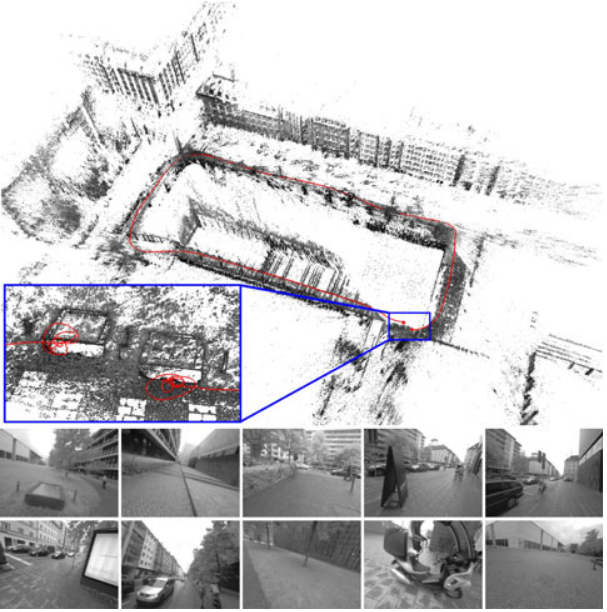
\includegraphics[width = 0.6\textwidth]{figures/dso_demo.png}
    \caption{DSO定位及建图效果\cite{engel2017direct}}
    \label{fig:dso_demo}
\end{figure}

\textbf{直接法}:
尽管特征点法在视觉SLAM中占据主流地位,
但其仍然具有计算时间长、不能充分利用图像中的信息以及依赖纹理信息等缺点,
直接法就是为了克服特征点法的上述缺点而存在的。
直接法根据像素的亮度信息估计相机的运动,
可以完全不用计算关键点和描述子,
于是,既避免了特征的计算时间,又避免了特征缺失的情况。
只要场景中存在明暗变化(可以是渐变,不必形成局部的图像梯度),直接法就能工作。
首个具有重要意义的直接法视觉SLAM方案是于2011年被提出来的DTAM\cite{newcombe2011dtam},
它是稠密单目视觉SLAM的先驱,并且在2015年的工作MobileFusion\cite{ondruvska2015mobilefusion}中适配到智能手机上。
2014年提出的LSD-SLAM\cite{engel2014lsd}是首次使用半稠密建图(semidense mapping)以适应大尺度环境的方法之一。
时间上更新一点的一个直接法方案是于2016年被提出的DSO\cite{engel2017direct},
这是一个构建稀疏地图以实现轻量化处理的直接法视觉里程计(Visual Odometry, VO),
其定位和建图效果如图\ref{fig:dso_demo}所示。
还有一种主要的视觉SLAM方法是于2017年被提出的半直接视觉里程计(Semidirect Visual Odometry, SVO)\cite{forster2016svo},
它结合了直接法和非直接法的优势。

\begin{figure}[htbp]
    \centering
    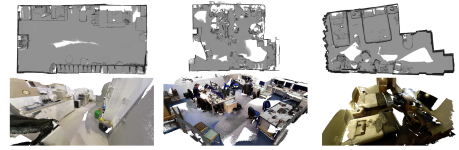
\includegraphics[width = \textwidth]{figures/elastic_fusion_demo.png}
    \caption{ElasticFusion三维重建效果\cite{whelan2015elasticfusion}}
    \label{fig:elastic_fusion_demo}
\end{figure}
\textbf{RGB-D法}:
RGB-D法视觉SLAM方法需要特制的硬件,即RGB-D相机,又称深度相机。
RGB-D相机除了获取环境的RGB图像外,还可以通过结构光和飞行时间(Time of Flight, ToF)等方式获取图像中每个像素点对应的环境中点深度(depth),
因此可以直接获得当前图像对应的稠密点云(point cloud),极大地方便了SLAM过程。
2011年提出的KinectFusion\cite{newcombe2011kinectfusion}目标就在于使用Microsoft Kinect深度相机对环境进行精细的三维重建。
Kerl等人于2013年提出的稠密视觉SLAM方法\cite{kerl2013dense}主要专注于利用稠密地图的优势进行精确定位。
Whelan等人于2015年提出了ElasticFusion\cite{whelan2015elasticfusion},该方法则更多地关注重建出的三维模型的几何精度。

(2)视觉惯性SLAM

\begin{figure}[htbp]
    \centering
    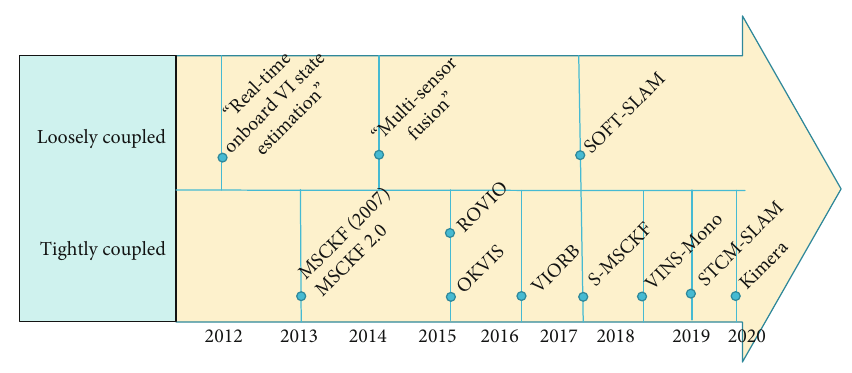
\includegraphics[width = \textwidth]{figures/vislam_classification.png}
    \caption{视觉惯性SLAM方法分类\cite{servieres2021visual}}
    \label{fig:vislam_classification}
\end{figure}

视觉惯性SLAM的引入主要是为了提高纯视觉SLAM系统的鲁棒性:
视觉传感器可以提供比较丰富的环境信息,但在绝对尺度的获取方面存在短板,并且图像获取频率较低,通常为几十Hz;
而惯性传感器可以精确感知自身运动,其测量数据天生携带尺度信息,并且数据获取频率较高,通常为几百Hz。
融合视觉和惯性传感器测量数据的SLAM方案则可以结合二者的优点。
视觉惯性SLAM也可以像视觉SLAM一样按输入信息分为直接法和非直接法,
但视觉惯性SLAM主要还是基于特征点法,
因此如图\ref{fig:vislam_classification}所示,
将视觉惯性SLAM按照视觉和惯性数据的耦合程度分为松耦合法(loosely-coupling methods)和紧耦合法(tightly-coupling methods)\cite{servieres2021visual}:

\textbf{松耦合法}:
松耦合法视觉惯性SLAM将IMU和图像测量数据分开来处理,并且使用二者的信息来跟踪位姿。
Weiss等人\cite{weiss2012real}通过对图像进行处理来计算连续位姿之间的视觉里程计,随后将后者与惯性测量数据融合。
也可以通过对IMU测量数据进行滤波来估计与基于图像的估计算法融合的旋转。
松耦合视觉惯性里程计(Visual-Inertial Odometry, VIO)也是2014年发表的一种全局多传感器融合(磁力计、气压计、GPS接收器、激光扫描仪等)方法\cite{shen2014multi}的一部分。
2017年发表的SOFT-SLAM\cite{cvivsic2018soft}算法则是一种在IMU可用时将其用来减小计算时间的方法,
它运行在无人机上并且可以实时构建稠密地图。

\begin{figure}[htbp]
    \centering
    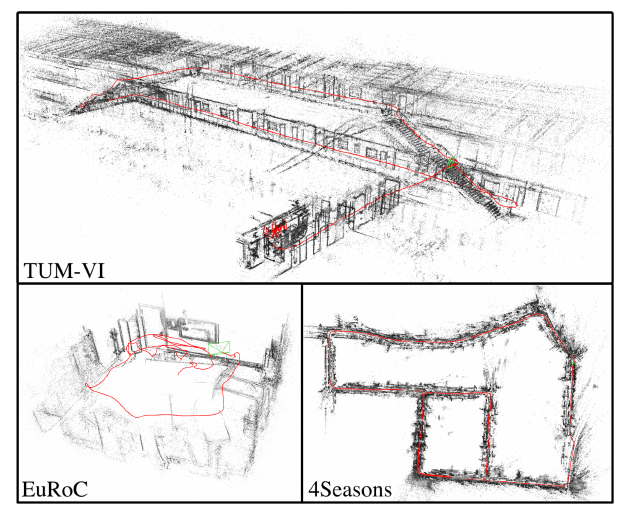
\includegraphics[width = 0.6\textwidth]{figures/dm_vio_demo.png}
    \caption{DM-VIO在3个基准数据集上的运行效果\cite{von2022dm}}
    \label{fig:dm_vio_demo}
\end{figure}

\textbf{紧耦合法}:
紧耦合法直接融合视觉和惯性传感器的原始测量数据来改善精度和鲁棒性,
而不是先使用基于视觉和基于惯性的估计算法分别对状态进行估计后再对二者结果进行融合。
MSCKF\cite{mourikis2007multi}和MSCKF 2.0\cite{li2013high}就属于紧耦合视觉惯性SLAM算法,二者都很鲁棒很轻量。
2015年提出的ROVIO\cite{bloesch2015robust}也是一种基于EKF的紧耦合直接法VIO。
著名的OKVIS\cite{leutenegger2015keyframe}和S-MSCKF\cite{sun2018robust}是双目VIO。
Lupton等人于2011年提出了IMU预积分(pre-integration)\cite{lupton2011visual},
可以显著降低基于优化的视觉惯性SLAM的计算量。
Foster等人于2016年对IMU预积分作出改进\cite{forster2016manifold},使其能更好地适应旋转群的流形结构。
基于改进后的IMU预积分方法,
Qin等人于2018年提出了VINS-Mono\cite{qin2018vins},VINS-Mono是一套真正的视觉惯性SLAM而非仅仅是一种VIO方法\cite{servieres2021visual}。
Kimera\cite{rosinol2020kimera}也是基于VIO的方法,但它同时还包含用于全局轨迹估计的多线程位姿图优化器、一个3D网格重建模块和一个3D度量-语义重建模块。
2021年发表并开源的ORB-SLAM3\cite{campos2021orb}是在纯视觉的ORB-SLAM2\cite{mur2017orb}的基础上融合了IMU数据,并引入地图拼接,提高了鲁棒性。
2022年发表的DM-VIO\cite{von2022dm}基于延迟边缘化(delayed marginalization)和位姿图光束平差法(pose graph bundle adjustment, PGBA)并将这两种技术用于IMU初始化,
这让DM-VIO的效果在视觉惯性里程计中达到了最高水平,其在3种公开的基准数据集上的表现见图\ref{fig:dm_vio_demo}。

\subsubsection{无人机的外力估计文献综述及简析}
在\ref{subsubsec:external_wrench_estimation}节中已经提到,
当前无人机的外力估计方法主要可分为确定性方法、概率性方法和基于滑窗优化的方法,
本小节接下来分别对这三类方法做文献综述及简析。

\textbf{确定性方法}:
确定性方法是通过将合推力向量从惯性测量数据中减掉来估计外力的\cite{tomic2014unified}。
这类方法主要是基于非线性观测器,包括扰动观测器(disturbance observer, DOB)\cite{liang2023active, yuksel2014nonlinear}、动量观测器(momentum observer, MOB)\cite{bodie2019omnidirectional,nigro2021control, tomic2016flying,ruggiero2014impedance}等。
确定性方法的缺点主要在于没有考虑推力输入、系统状态和IMU的噪声,也没有考虑IMU的时变零漂。
因此,确定性方法只有在输入输出数据经过仔细处理过或者所用的传感器的信噪比非常高的情况下才能正常工作。

\textbf{概率性方法}:
概率性方法主要基于卡尔曼滤波。
考虑到基于非线性观测器方法对噪声敏感的特性,
McKinnon等人于2011年提出了一种基于无迹卡尔曼滤波(Unscented Kalman Filter, UKF)的无人机合外力和外力矩估计算法\cite{mckinnon2016unscented},
该方法显著提高了外力估计的效果。
类似的基于滤波的方法还有:
2013年Augugliaro等人提出的一种基于卡尔曼滤波的外力估计方法\cite{augugliaro2013admittance},该方法面向人与四旋翼无人机的物理交互;
2016年Tagliabue等人提出的一种基于UKF的外力估计方法\cite{tagliabue2016collaborative},该方法面向无人机的协同物品运输。
这些方法都可以归类为松耦合方法,
因为它们对系统状态的估计来源于一个分立的估计器,
随后在另一个分立的估计步骤中将这个估计结果与来自无人机动力学模型的预测融合。
松耦合估计器没有考虑所有待估计变量之间的关联,这可能会导致估计结果不精确。
此外,对外力的估计是在一个额外的融合步骤中进行的,这可能会带来延迟和额外的计算负担\cite{nisar2019vimo}。

\begin{figure}[!ht]
    \setlength{\subfigcapskip}{-1bp}
    \centering
    \begin{minipage}{\textwidth}

    \centering
    \subfigure{\label{subfig:vimo_factor_graph}}\addtocounter{subfigure}{-2}
    \subfigure{\subfigure[VIMO的因子图\cite{nisar2019vimo}]{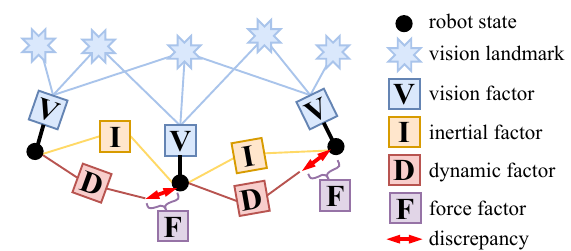
\includegraphics[width=0.45\textwidth]{vimo_factor_graph.png}}}
    \subfigure{\label{subfig:vid_fusion_factor_graph}}\addtocounter{subfigure}{-2}
    \subfigure{\subfigure[VID-Fusion的因子图\cite{ding2021vid}]{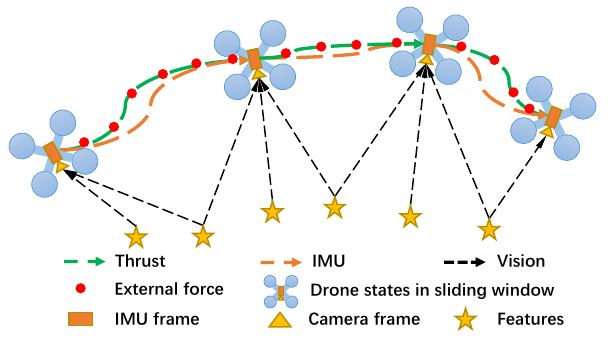
\includegraphics[width=0.45\textwidth]{vid_fusion_factor_graph.png}}}

    \end{minipage}
    \caption{两种视觉-惯性-动力学里程计的因子图}
    \label{fig:common_sensors_for_slam}
\end{figure}

\textbf{基于滑窗优化的方法}:
目前基于滑窗优化的无人机外力估计方法主要是将动力学模型应用到VIO系统中。
Antonini的研究\cite{antonini2018pre}表明,
在基于平滑的VIO中,
将动力学残差结合IMU残差作为加速度信息的额外来源可以增加状态估计的鲁棒性,
尤其是在加速度计信噪比低的低速飞行场景中。
但Antonini的方法只建模了空气阻力,而忽略了其他外力作用,
这在有风或者外力作用的场景下可能会造成系统对IMU零漂和外力的混淆,导致对零漂的错误处理\cite{abeywardena2014model},
因此该方法只能在无扰动的环境中运行。
Kobilarov等人于2015年提出了一种基于动态微分规划(Dynamic Differetial Programming, DDP)的状态和外力估计方法\cite{kobilarov2015differential},
但该方法对测量过程过于简化而没有展示出实际应用价值。
Nisar等人于2015年提出了能同时估计运动和外力的视觉里程计VIMO\cite{nisar2019vimo},
该方法是一个第一个基于优化的视觉-惯性-动力学紧耦合估计器,
它以视觉、惯性的测量数据以及合推力指令为输入,
将合推力指令作预积分用作构造动力学残差,并将动力学残差加入到VINS-Mono\cite{qin2018vins}的滑窗优化的代价函数中,
得到如图\ref{subfig:vimo_factor_graph}所示的因子图。
实验结果表明VIMO在状态估计方面相比原始的VINS-Mono在准确度上有最高可达29\%的提升,
同时在不增加计算时间的情况下还能提供对外力的估计。
VIMO搭起了在基于优化的VIO系统中运动估计和外力估计之间的桥梁,
但是由于将外力建模为零均值的Gaussian,
VIMO在较大或连续的外力作用下会受到严重影响甚至会失效\cite{ding2021vid}。
为解决VIMO的上述问题,
Ding等人于2021年提出了VID-Fusion\cite{ding2021vid},
VID-Fusion是一个完整的基于优化的紧耦合视觉-惯性-动力学里程计,
其因子图如图\ref{subfig:vid_fusion_factor_graph}所示,
它在VIMO的基础上增加了外力预积分项来表示外力对无人机的作用;
无人机的合推力信息来自于自制的转速测量单元(Rotating speed Measurement Unit, RMU),
每个RMU对旋翼电机磁场进行测量,
将该测量数据进行快速傅里叶变换(Fast Fourier Transform, FFT)后可得到每个旋翼的转速值,
再结合辨识出的旋翼升力系数可得到合推力。
由于VID-Fusion显式考虑了外力的影响,
即使是在外力变化范围很大的情况下它也具有与VINS-Mono和VIMO相当甚至更好的精度。
不过VIMO和VID-Fusion都只能估计3轴合外力,而不能估计外力矩。
除了基于视觉惯性里程计的方法外,
2022年Papadimitriou等人还提出了一种基于非线性滚动时域估计(Non-linear Moving Horizon Estimation, NMHE)的无人机状态和外力估计方法\cite{papadimitriou2022external},
该方法配合非线性模型预测控制(Non-linear Model Predictive Control, NMPC),
实现了无人机对各种外部干扰的补偿,
该方法同样只估计了合外力而没有估计外力矩。

\subsubsection{全驱动旋翼无人机文献综述及简析}
\textbf{固定旋翼型}:
固定旋翼型过(全)多旋翼飞行器的机械结构相对简单,飞行器通过改变不同朝向旋翼的转速来控制推力和转矩的大小和方向。
如图\ref{subfig:fix_rotor}所示为Brescianini等人于2016年发表的一种实现灵活全向飞行的固定旋翼型八旋翼飞行器系统\cite{brescianini2016design},
该系统采用8个可逆电机-旋翼组合执行器(reversible motor-propeller actuator),故每个执行器都可以产生正推力和负推力,
8个执行器的构型是基于静态力和扭矩分析,采用求解优化问题的方式来设计的,以期最大化飞行器的灵活性并最大限度保证飞行器动力学特性的旋转不变性。
不过,固定旋翼型的冗余驱动飞行器的一个主要缺点在于:这些旋翼通常不会同时直接朝向竖直方向,使得这类飞行器的悬停效率不会很高;
并且如果设定旋翼朝向使之更倾向于高效的悬停和更高的有效载荷,就会几乎不可避免地降低产生横向作用力的能力\cite{allenspach2020design}。

\begin{figure}[ht]
    \centering
    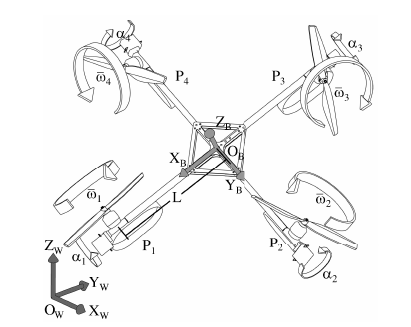
\includegraphics[width = 0.65\textwidth]{omni_quadrotor.png}
    \caption{Markus Ryll等人的可倾转旋翼的全向四旋翼飞行器结构示意图}
    \label{fig:tiltrotor_quadrotor}
\end{figure}

\textbf{倾转旋翼型}:
倾转旋翼型全向多旋翼飞行器的实现方式多数是为旋翼增加额外的自由度,使其转轴指向可以改变。
比较常用的方式是为安装旋翼的机臂添加一个绕其轴的旋转自由度:
如图\ref{fig:tiltrotor_quadrotor}展示了Markus等人于2015年研制出的一种可倾转旋翼的冗余驱动四旋翼飞行器的结构\cite{ryll2014novel},该飞行器可以在有限的横滚角和俯仰角下实现悬停;
图\ref{subfig:tilt_rotor}展示的是Kamel等人于2018年开发的一种可倾转旋翼的全向六旋翼飞行器Voliro\cite{kamel2018voliro},该飞行器可以实现任意姿态下的悬停和飞行。
这类飞行器通过改变每个旋翼的朝向,实现了更高效的悬停。
本课题所使用的仿真及实物实验平台是参考Voliro的结构搭建的。

\begin{figure}[!ht]
    \setlength{\subfigcapskip}{-1bp}
    \centering
    \begin{minipage}{\textwidth}

    \centering
    \subfigure{\label{subfig:trajectory_overview}}\addtocounter{subfigure}{-2}
    \subfigure{\subfigure[规划出的6自由度轨迹示意图]{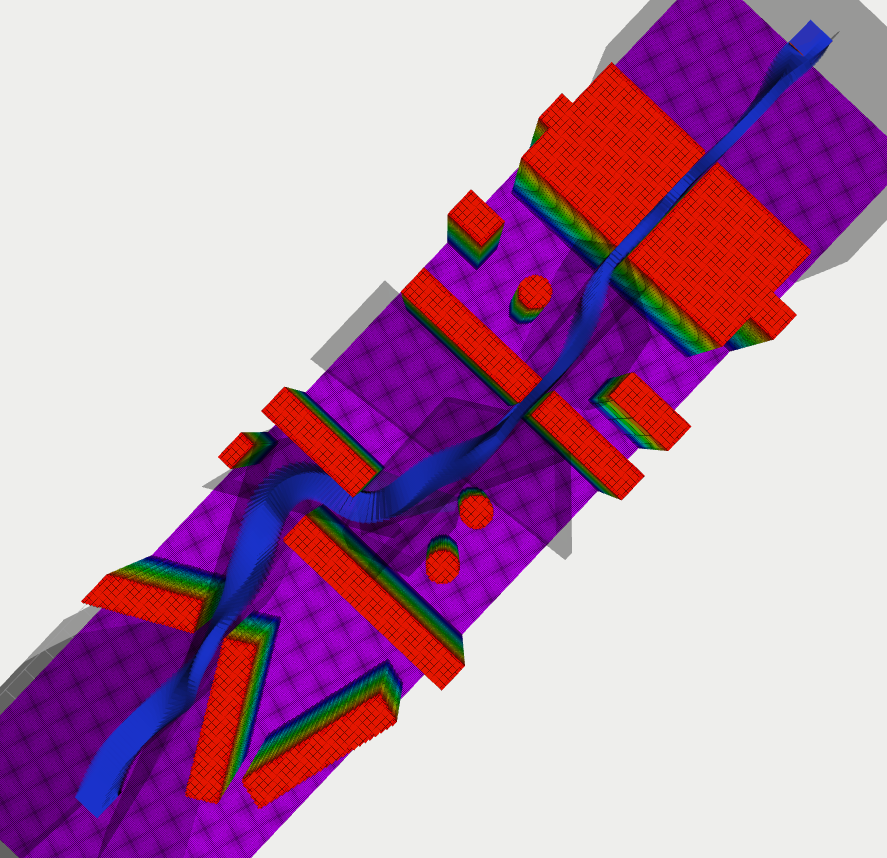
\includegraphics[width=0.45\textwidth]{sfc_and_traj.png}}}
    \subfigure{\label{subfig:simulation}}\addtocounter{subfigure}{-2}
    \subfigure{\subfigure[仿真结果示意图]{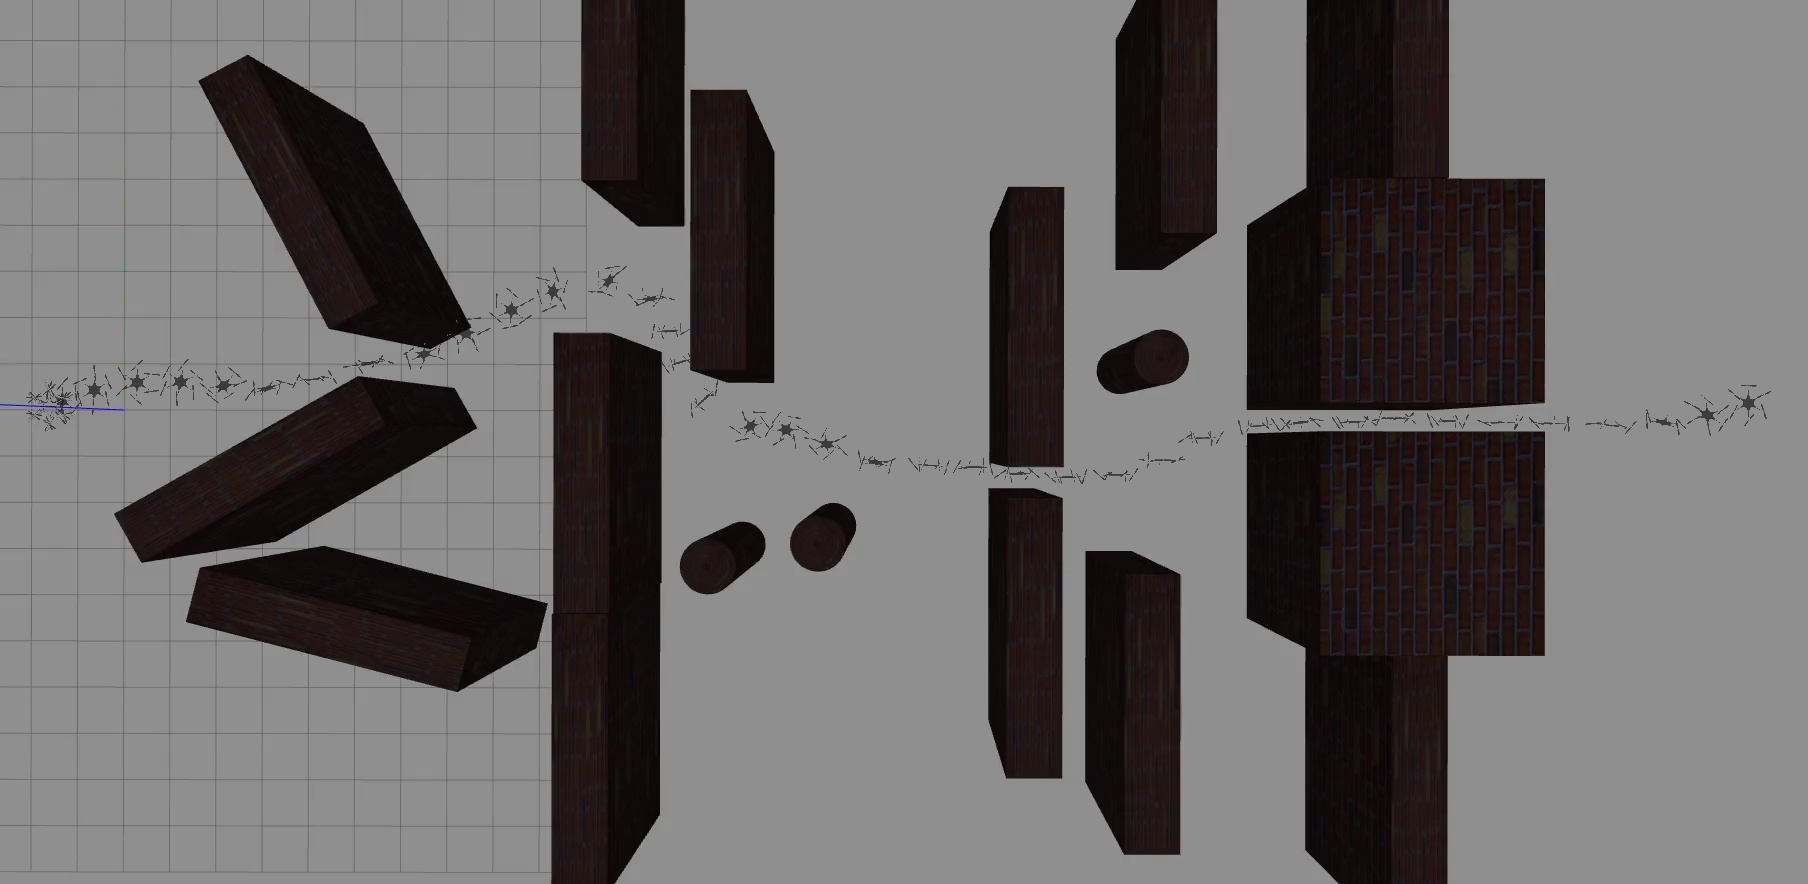
\includegraphics[width=0.45\textwidth]{complex_env_simulation.jpg}}}

    \end{minipage}
    \caption{无碰撞6自由度轨迹规划示意图\cite{liu2022collision}}
    \label{fig:collision_free_6dof_trajectory}
\end{figure}

目前关于全驱动无人机的研究处于起步阶段,
现有工作主要关注机械结构和控制算法,
而针对全驱动无人机导航的研究则非常稀少,
仅有部分为全驱动无人机设计运动规划算法的工作。
2018年Brescianini等人基于运动基元为全向飞行器生成了从给定起点到给定终点且满足一定输入约束的6自由度轨迹\cite{brescianini2018computationally},该工作可以在短时间内迅速探索出大量轨迹并判断其可行性。
同年Morbidi等人提出了用于倾转旋翼六旋翼飞行器的节能轨迹生成方法\cite{morbidi2018energy},通过求解一个显式考虑电机电气模型的优化控制问题得到一条指定边界点的节能轨迹,并做了数值验证。
2021年Pantic等人提出了基于流形网格的运动规划方法\cite{pantic2021mesh},该方法将物体表面(surface)建模为三角网格(triangular mesh)并提出原始表面的一个低维参数化表示方法,进一步将原始表面及其低维表示近似为流形(manifold),运用黎曼运动策略(Riemannian Motion Policies,RMPs)构建了一个高效且通用的、面向飞行器与表面交互的运动规划框架。
2022年Liu等人为全驱动无人机提出了一种6自由度时间最优轨迹的生成方法\cite{liu2022optimal}。
以上工作无一例外都没有将环境中的障碍物纳入考虑。
2022年本课题组提出了一种基于优化的全驱动飞行器6自由度无碰撞轨迹生成方法\cite{liu2022collision},
该方法将Wang等人于2022年提出的MINCO轨迹类及基于MINCO的几何约束多旋翼轨迹优化框架GCOPTER\cite{wang2022geometrically}扩展到了6维,
并且考虑了机器人的几何形状和姿态,
因此生成的轨迹可以充分利用环境中的无碰撞空间,
使得无人机安全穿越狭长空间成为可能,
具体效果如图\ref{fig:collision_free_6dof_trajectory}所示。
还有部分为针对6自由度刚体运动规划的工作
\cite{nguyen2016time, belta2002svd, belta2002euclidean, bestaoui2003motion, zefran1998generation, watterson2016smooth, jackson2021planning}
具有应用到全驱动无人机上的可能。

\section{主要研究内容及研究方案}
\subsection{研究内容}
本课题主要对多旋翼无人机的视觉-惯性导航方法进行研究,
期望能设计一个能在实现精确的运动估计的同时,
还能将欠驱动无人机和全驱动无人机的动力学模型纳入考虑以得到精确实时的合外力和外力矩估计的视觉-惯性导航系统,
并期望能将该导航系统部署到全驱动无人机上,
配合稠密建图和运动规划算法实现全驱动无人机在未知复杂环境下的自主导航并提高其抗扰性能。

\subsubsection{应用动力学模型的视觉惯性里程计的研究}
目前基于视觉惯性的紧耦合无人机外力估计方案只能对欠驱动无人机的3维合外力进行估计,不能适用与全驱动无人机,也不能估计外力矩。
外力矩相关的角加速度并不能通过传感器直接获得,
直接对陀螺仪测量的角速度值进行差分可能会引入额外噪声\cite{邱国鹏2023应用视觉}。
已有的可估计外力矩的方法主要基于非线性观测器和卡尔曼滤波,
多数属于松耦合方法,
且存在对噪声敏感,或引入延迟和额外的计算量的问题。
本课题尝试对视觉惯性导航和外力估计的理论进行研究,
结合各种方法的优点和思想,
设计一种基于视觉惯性的可精确、鲁棒且实时地同时估计无人机运动、外力和外力矩的导航方案。

% \subsubsection{全驱动无人机的研究}
% 本课题期望能将所设计的视觉惯性导航系统部署到全驱动无人机上,
% 实现全驱动无人机的自主导航。
% 首先需要对全驱动无人机的机械结构和理论模型进行了解,
% 特别是全驱动无人机的动力学模型和控制策略,
% 本课题将基于全驱动无人机OmniHex的仿真和实物平台对此展开研究。

\subsubsection{无人机稠密地图构建及运动规划方法的研究}
本课题要实现无人机的自主导航,
除主要研究内容视觉惯性里程计外,
还需要对稠密建图和运动规划算法进行研究,
其中欠驱动无人机需要为其规划3自由度的平移运动,全驱动无人机需要为其规划6自由度的刚体运动。
本课题将对基于RGB-D相机的稠密建图和复杂环境中全驱动无人机的运动规划方案进行研究设计。

\subsubsection{全驱动无人机自主导航的研究}
本课题最后将结合全驱动无人机的特点,把前述状态估计、建图和规划模块整合为一个完整的无人机自主导航系统,
部署到全驱动无人机上,
实现全驱动无人机的自主导航。

\subsection{研究方案}
\subsubsection{应用动力学模型的视觉惯性里程计的研究方案}
本课题首先将对最优估计、计算机视觉和无人机系统建模等相关理论知识进行学习研究。
对现有不同的VIO、外力估计方案进行调研和对比,
总结各方法的主要思想、优势和短板,
选择合适的外力矩估计方式,
构建相关数学模型,
设计相关算法
并尝试针对研究对象的特点进行理论创新。
然后在已有的算法框架基础上进行修改,
或者开发自己的算法框架。

由于当前OmniHex的软件系统和仿真平台是主要基于ROS2开发的,
并且ROS2在各方面相对于ROS更有优势,
因此本课题的导航系统考虑基于ROS2实现,
考虑到目前主流的视觉惯性导航框架都是基于ROS实现的,
因此本课题的工程实现可能涉及算法移植。
具体选择哪个平台有待后续调研。
为得到无人机的推力信息,
除参考VIMO直接使用飞控输出的推力指令外,
更好的解决方案可能是参考VID-Fusion自制RMU,
因此可能涉及嵌入式开发。

最后分别进行仿真和实物实验进行验证。
其中同时估计外力的VIO算法还将基于公开数据集进行验证,
该算法的实物验证计划分别基于欠驱动无人机和全驱动无人机进行实验,
外力的来源计划使用弹性绳、风扇、悬挂负载等,
其中弹性绳生成的外力真值可通过力传感器获取。

\subsubsection{全驱动无人机稠密地图构建及运动规划方法的研究方案}
一个完整的无人机自主导航框架除了包括定位模块外,
还包括建图和规划模块。
本课题还将对稠密地图构建和运动规划方法进行研究。
对于全驱动无人机而言,
需要为其规划无碰撞的6自由度刚体运动,
这方面此前已有研究基础,
本课题中将对之前的工作进行进一步研究和改进。
考虑到运动规划部分的需要,
本课题将主要对稠密点云地图、占据栅格地图和ESDF地图的构建方法进行研究,
最终目的是要能方便地基于地图进行碰撞检测、路径搜索和安全飞行走廊生成。
这方面已有许多成熟的开源框架可以直接使用,
本课题将基于成熟框架进行必要的二次开发和创新。

\subsubsection{无人机自主导航的研究方案}

\begin{figure}[ht]
    \centering
    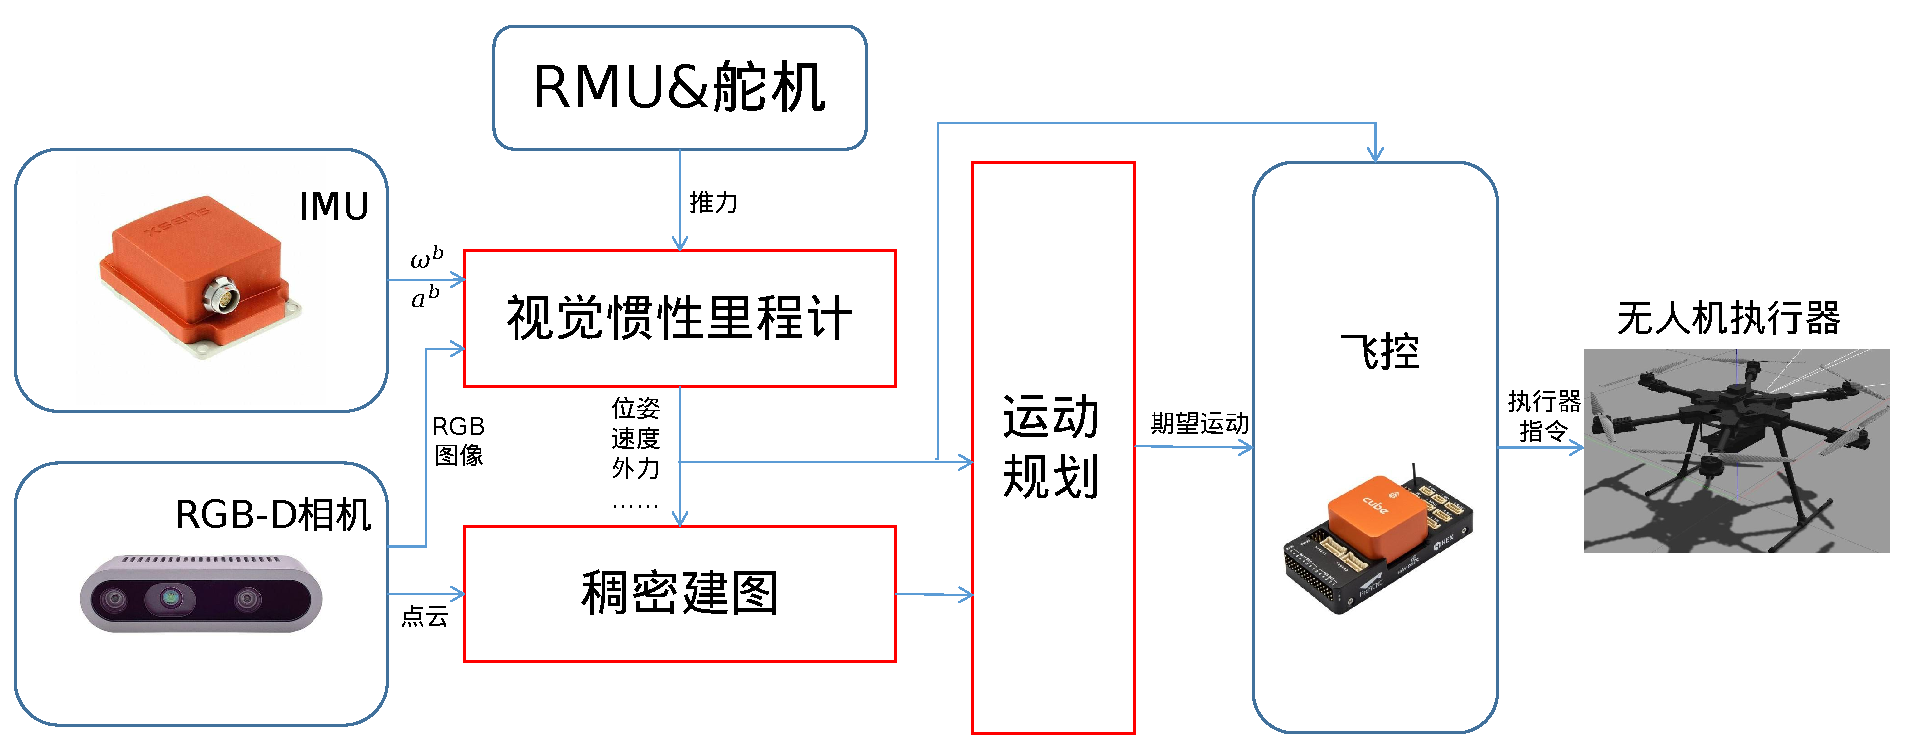
\includegraphics[width = \textwidth]{navigation_system.pdf}
    \caption{自主导航系统框架图}
    \label{fig:navigation_system}
\end{figure}

这一部分将主要是工程实现的工作,
包括传感器的选型和部署、各模块的整合等。
传感器方面,
视觉传感器计划使用RGB-D相机, 
它可以输出双目的RGB图像和对应的相机坐标系下的稠密点云,
双目RGB图像用于视觉惯性里程计,
稠密点云用于稠密建图;
惯性测量方面可直接使用Pixhawk飞控自带的IMU。
对于外力估计时需要的无人机的推力信息,
除参考VIMO直接使用飞控输出的推力指令外,
更好的解决方案可能是参考VID-Fusion自制RMU,
因此可能涉及嵌入式开发;
对于全驱动飞行器而言还需要获取旋翼倾转舵机的转角,
这里直接用飞控输出的控制指令即可。
在传感器部署的时候需要考虑全驱动无人机的结构和运动的特点,
科学选取传感器的数量和部署方式。
整个自主导航系统架构的初步设计方案如图\ref{fig:navigation_system}所示。

本课题涉及软硬件开发与调试等工程问题。
由于当前OmniHex的软件系统和仿真平台是主要基于ROS2开发的,
并且ROS2在各方面相对于ROS更有优势,
因此本课题的导航系统考虑基于ROS2实现,
考虑到目前主流的视觉惯性导航框架都是基于ROS实现的,
因此本课题的工程实现可能涉及算法移植。
具体选择哪个平台有待后续调研。
目前OmniHex的实物模型还不能做到大倾角飞行,
需要进行进一步调试,
如有必要需修改机械结构或者搭建一台新飞机。

\section{预期目标}
本课题的目标是设计一个基于视觉惯性融合的SLAM导航系统,
期望此系统能够:

(1)精确且高效地估计自身运动。

(2)能结合无人机的动力学模型精确且高效地估计外部作用力。
 
(3)适用于全驱动无人机,并能结合建图与规划算法实现自主导航。

\section{已完成的研究工作及进度安排}
\subsection{已完成的研究工作}
2021年9月至2022年6月:
协助搭建了OmniHex仿真和实物平台,
并设计了一种面向全驱动无人机的6自由度无碰撞轨迹生成算法。

2022年6月至2023年6月:
系统学习最优估计、最优控制、移动机器人导航、计算机视觉等基础专业知识,
调研了视觉定位、运动规划相关论文。

2023年6月至2023年9月:
调研学习视觉及视觉惯性SLAM相关文献,
系统学习VINS-Mono的理论和代码。

\subsection{进度安排}
本课题的研究从2023年9月开始,到2024年12月进行最终答辩,
结合自身知识储备和科研学习能力,制定如下进度安排:

2023年9月至2023年11月:
调研学习视觉惯性导航和无人机外力估计的理论方法,
总结已有方法的优缺点和设计思想,
对相关理论进行具体研究。
同时对OmniHex实物平台进行调试。

2023年11月至2024年4月:
完成同时估计运动和外力的视觉惯性里程计算法的设计和实现
并完成在公开数据集和仿真中完成基于欠驱动和全驱动飞行器的验证。

2024年4月至2024年7月:
完成稠密建图和运动规划算法的设计和实现,
并配合VIO实现首先完成基于四旋翼无人机的仿真和实验验证。

2024年7月至2024年8月:
完成基于OmniHex的自主导航仿真实验。

2024年8月至2024年10月:
完成基于OmniHex的自主导航实物实验。

2024年10月至2024年12月:
撰写论文。

\section{已具备的研究条件和所需条件及经费}
\subsection{实验室条件和经费保障}
实验室已有多架四旋翼无人机、一架OmniHex和一套动作捕捉系统,
传感器、电机和计算设备种类其全数量足够,
全驱动无人机属于实验室项目,经费足够,
可满足本课题的基本需求。

\subsection{所需条件及经费}
本课题所需经费主要在于全驱动无人机的实物搭建上,
目前已有的OmniHex各部分估计造价如表\ref{tab:omni_hex_bom}所示:

\begin{table}[htbp]
    \caption{OmniHex主要组件BOM表\label{tab:omni_hex_bom}}
    \vspace{0.5em}\centering\wuhao
    \begin{tabular}{ccccccc}
    \toprule[1.5pt]
    组件名称 & 预估单价 & 数量 & 总额 \\
    \midrule[0.2pt]
    Intel NUC 迷你计算机 & 4000 & 1 & 4000 \\
    Pixhawk自驾仪 & 2000 & 1 & 2000 \\
    锂电池 & 70 & 1 & 70 \\ 
    固定起落架 & 100 & 1 & 100 \\ 
    Dynamixel伺服舵机 & 2400 & 6 & 14400 \\
    无刷电机及相关配件 & 600 & 6 & 3600 \\ 
    电子配件 & 600 & $\backslash$ & 600 \\
    机架板材 & 700 & $\backslash$ & 700 \\ 
    轴承相关 & 1320 & $\backslash$ & 1320 \\
    紧固件 & 50 & $\backslash$ & 50 \\ 
    合计 & $\backslash$ & $\backslash$ & 26840 \\
    \bottomrule[1.5pt]
    \end{tabular}
  \end{table}

\section{预计困难及解决方案}
\subsection{预计困难与技术难点}
课题进行需要学习的知识较多,
涉及软硬件开发与调试、最优估计、计算机视觉、最优控制等知识;
研究过程涉及理论研究、工程实现等具有挑战性的步骤,
总体难度和工作量比较大。
预计可能遇到的困难如下:

(1)目前没有基于视觉-惯性的紧耦合外力矩估计方法,
而且与外力矩观测直接相关的角加速度无法直接从传感器中获得,
直接对角速度进行差分可能会引入额外噪声从而影响估计精度。

(2)目前OmniHex实物飞行器仅能进行小倾角(约$30^\circ$以内)姿态控制,
倾角过大会造成整个系统振荡发散导致坠机。
推测是由PID参数没有整定到位,以及舵机和机臂之间的传动结构存在的死区造成的,
后续由可能需要修改机械结构重新搭建一台OmniHex。

(3)全驱动无人机属于新兴领域,
在设计、控制和调试方面可借鉴经验极少,
全驱动无人机的自主导航更是未见先例,
因此本课题基于全驱动无人机的实物验证部分存在较大挑战性和不确定性。

\subsection{解决方案}
为了提高课题进展速度和效率,保证学习质量,
采用边应用边学习再应用的方法进行主要知识的系统学习,
并多动手实际操作,提高动手操作能力,也为后期打下良好的基础。
同时采取以下方案:

(1)广泛调研各种外力估计方案,
总结各方案的优势短板和设计思想,
集思广益,充分结合各种方案的优点。

(2)与实验室同窗以及老师多沟通多讨论,
寻找问题解决的思路和灵感,
遇到难以解决的问题及时向他人寻求帮助。
与同组人员合作学习,提高效率并避免重复性工作。

(3)理论学习与实践操作并行,
提高学习和工作效率。

\bibliographystyle{hitszthesis}
\bibliography{reference}

% Local Variables:
% TeX-master: "../report"
% TeX-engine: xetex
% End:
% \section{课题来源及研究的目的和意义}
\subsection{研究背景}
进入21世纪以来,多旋翼无人机领域取得了很大的发展,成为一类成功从实验室走进人们生活的机器人系统。
为突破现在市场上主流的欠驱动无人机所存在的瓶颈,近年来人们又研制出了不少种类冗余驱动多旋翼无人机系统。
作为一种全驱动系统,这种无人机可以跟踪6自由度轨迹,有效增强了多旋翼无人机的机动性能,拓宽了其应用场景。

作为一个高自由度且敏捷的系统,无人机的稳定自主飞行依赖一个鲁棒且高精度的导航系统来对自身和外界的状态进行有效估计。
同时定位与建图(Simultaneous Localization and Mapping, SLAM)技术被广泛应用于移动机器人的实时定位导航中,
使得无人机在复杂的无GPS环境中也能获得准确的状态估计和环境感知。
其中,基于视觉或视觉惯性融合的SLAM导航技术以其相对较低的成本、轻量级的硬件需求和可观的表现成为更适用与无人机的选择,
并且一直以来都是研究的热点。\cite{ding2021vid}
\subsection{研究的目的及意义}
\section{国内外研究现状及分析}
\subsection{国内外研究现状}
\subsubsection{视觉惯性导航研究现状}
\subsubsection{无人机的外力估计研究现状}
\subsubsection{全驱动旋翼无人机研究现状}
\subsection{国内外文献综述及简析}
\subsubsection{视觉惯性导航文献综述及简析}
\subsubsection{无人机的外力估计文献综述及简析}
\subsubsection{全驱动旋翼无人机文献综述及简析}

% Local Variables:
% TeX-master: "../report"
% TeX-engine: xetex
% End:
% \section{主要研究内容及研究方案}
\subsection{研究内容}
\subsection{研究方案}
% \section{预期目标}
\subsection{预期目标}
% \section{已完成的研究工作及进度安排}
\subsection{已完成的研究工作}
\subsection{进度安排}
% \section{已具备的研究条件和所需条件及经费}
\subsection{实验室条件和经费保障}
\subsection{所需条件及经费}
% \section{预计困难及解决方案}
\subsection{预计困难与技术难点}
\subsection{解决方案}

% 威海校区本科生开题报告结构 ----------------------------------------
% \input{body/report_weihai_bachelor_opening}
% \makebackcover
% -------------------------------------------------------------

% 威海校区本科生中期报告结构 ----------------------------------------
% \input{body/report_weihai_bachelor_midterm}
% \makebackcover
% -------------------------------------------------------------

% 哈尔滨校区本科生开题报告结构 --------------------------------------
% \section{课题来源及研究的目	的和意义}
(正文  宋体小4号字,行距1.25倍,段前0行,段后0行)
\section{国内外在该方向的研究现状及分析}
\section{主要研究内容}
\section{研究方案}
\section{进度安排,预期达到的目标}
\section{课题已具备和所需的条件、经费}
\section{研究过程中可能遇到的困难和问题,解决的措施}
\section{主要参考文献}
\cite{ding2021vid}
\bibliographystyle{hithesis}
\bibliography{reference}

% Local Variables:
% TeX-master: "../mainart"
% TeX-engine: xetex
% End:
% -------------------------------------------------------------
% \bibliographystyle{hithesis}
% \bibliography{reference}

\end{document}

% Local Variables:
% TeX-engine: xetex
% End:
